%%%%%%%%%%%%%%%%%%%%%%%%%%%%%%%%%%%%%%
%%%%%%%%%%%%%%%%%%%%%%%%%%%%%%%%%%%%%%
% Do not edit the TeX file your work
% will be overwritten.  Edit the RnW
% file instead.
%%%%%%%%%%%%%%%%%%%%%%%%%%%%%%%%%%%%%%
%%%%%%%%%%%%%%%%%%%%%%%%%%%%%%%%%%%%%%
  


We demonstrate the local sensitivity computations on a 
Gaussian mixture model of the iris dataset. 
The generative model and variational approximation were detailed in 
\exref{iris_bnp_process,iris_var_distr}, respectively. 
\figref{iris_fit} shows the GMM fit at $\alpha = 6$. 
The data consists of three iris species, and
the BNP model correspondingly identifies three dominant clusters. 


\begin{knitrout}
\definecolor{shadecolor}{rgb}{0.969, 0.969, 0.969}\color{fgcolor}\begin{figure}[!h]

{\centering 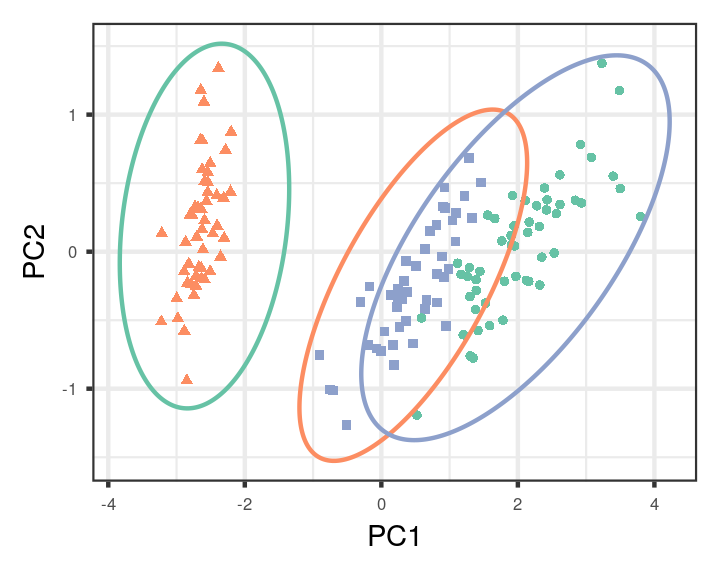
\includegraphics[width=0.588\linewidth,height=0.470\linewidth]{figure/iris_fit-1} 

}

\caption[The iris data in principal component space and 
                      GMM fit at $\alpha = 6$]{The iris data in principal component space and 
                      GMM fit at $\alpha = 6$. 
                      Colors denote inferred memberships and
                      ellipses are estimated covariances. }\label{fig:iris_fit}
\end{figure}


\end{knitrout}

We wish to evaluate the sensitivity of the expected number of clusters to the 
stick-breaking distribution. 
Define the expected number of \textit{in-sample} clusters as
\begin{align*}
\gclusters(\eta) &= \expect{\q(\z\vert\eta)}{\sum_{k=1}^\kmax \ind{ \sum_{n=1}^{N}
\z_{\n\k} > 0}} \\ 
&= \sum_{k=1}^\kmax \left(1 -  \prod_{n=1}^N
\left(1 - \expect{\q(\z_{nk}\vert\eta)}{\z_{nk}}\right)\right).
\end{align*}
Recall that the expectation and product can be interchanged because $q$ is mean-field. 

The in-sample quantity $\gclusters$ is an estimate for 
the number of species present in the observed iris dataset. 
Alternatively, we can define a {\itshape posterior predictive} quantity, 
which is an estimate of the number of species one would expect to see 
should a new iris dataset of size $N$ be collected.
Define the posterior predictive number of clusters as 
\begin{align}\eqlabel{post_pred_nclusters}
\gclusterspred(\eta) = \expect{\q(\nu\vert\eta)}{\sum_{k=1}^\kmax\left(1 -
(1 - \pi_k)^N\right)},
\end{align}
where recall that $\pi_k$ are the mixture weights computed from the stick-lengths, $\pi_\k = \nuk \prod_{\k' < \k} (1 - \nu_{\k'})$. 

Unlike the in-sample quantity, the expectation for the predictive quantity is not a simple closed-form function of the variational parameters.  
Instead, we approximate~\eqref{post_pred_nclusters} using Monte Carlo draws from the variational distribution. 
Specifically, we use the ``reparameterization trick" to sample from the variational distribution:
we use an appropriately chosen, $\eta$-dependent transformation 
$f(\cdot, \eta)$ that satisfies 
\begin{align*}
  u \iid\normdist{0, I} \implies 
  f(u, \eta) \stackrel{d}{=} \nu \sim \q(\cdot | \eta).
\end{align*}
To form a Monte Carlo estimate of \eqref{post_pred_nclusters}, 
we sample $u_1, ..., u_m\stackrel{iid}{\sim}\normdist{0, I}$ 
and then average the expression inside the expectation evaluated at points 
$f(u_1, \eta), ..., f(u_m, \eta)$.
We use the reparameterization trick so that conditional on $u_1, ..., u_m$,
our Monte Carlo estimate of $\gclusterspred$ is a determinstic function of 
the variational parameters $\eta$. 
In our experiments below, all displayed values of $\gclusterspred(\eta)$ are
Monte-Carlo approximations, 
conditional on the same $m = 10,000$ draws $u_1, ..., u_m$, fixed a priori. 

We evaluate the sensitivity of the posterior quantities 
$\gclusters$ and $\gclusterspred$ to the prior parameter $\alpha$. 
We first fitted the initial approximate posterior at $\alpha_0 = 6$. 
Subsequent refits at $\alpha\not=\alpha_0$ used the variational parameters
$\etaopt(\alpha_0)$ as an initialization. 
As $\alpha$ increases, both the expected in-sample and the expected predictive number of clusters increases (\figref{iris_alpha_sens}). 
The in-sample quantity is relatively insensitive to changes in the $\alpha$ parameter. 
As $\alpha$ varies from $\alpha = 1, ..., 16$,
the quantity $\gclusters(\etaopt(\alpha))$
varies only from 
3.0 to
3.4
(recall that the true number of iris species is three). 
On the other hand, the posterior preditive quantity is sensitive 
to changes in $\alpha$.
Over the same range of $\alpha$, $\gclusterspred(\etaopt(\alpha))$
varies from 
3.6 to 
8.1. 

We constructed the linear approximation at $\alpha = 6$ and computed
the approximate variational parameters $\etalin(\alpha)$ at 
$\alpha = 1, ..., 16$. 
Substituting $\etalin(\alpha)$ for $\etaopt(\alpha)$, 
we observe that $g(\etalin(\alpha))$ is able to mimic the changes 
in both the in-sample and predictive quantities 
found by refitting the model (\figref{iris_alpha_sens}).  
Furthermore, the linear approximation is an order of magnitude faster than refitting. 
Forming the linear approximation, which requires a Hessian inversion (\eqref{vb_eta_sens}), required 0.02 seconds. 
After forming the linear approximation at $\alpha = 6$,
computing $\etalin(\alpha)$ for all $\alpha = 1, ... 16$ took another 
0.02 seconds.
On the other hand, to refit $\etaopt(\alpha)$ for the same range of
$\alpha$'s took a total of 10 seconds, 
with a median refit time of 0.7 seconds. 









\begin{knitrout}
\definecolor{shadecolor}{rgb}{0.969, 0.969, 0.969}\color{fgcolor}\begin{figure}[!h]

{\centering 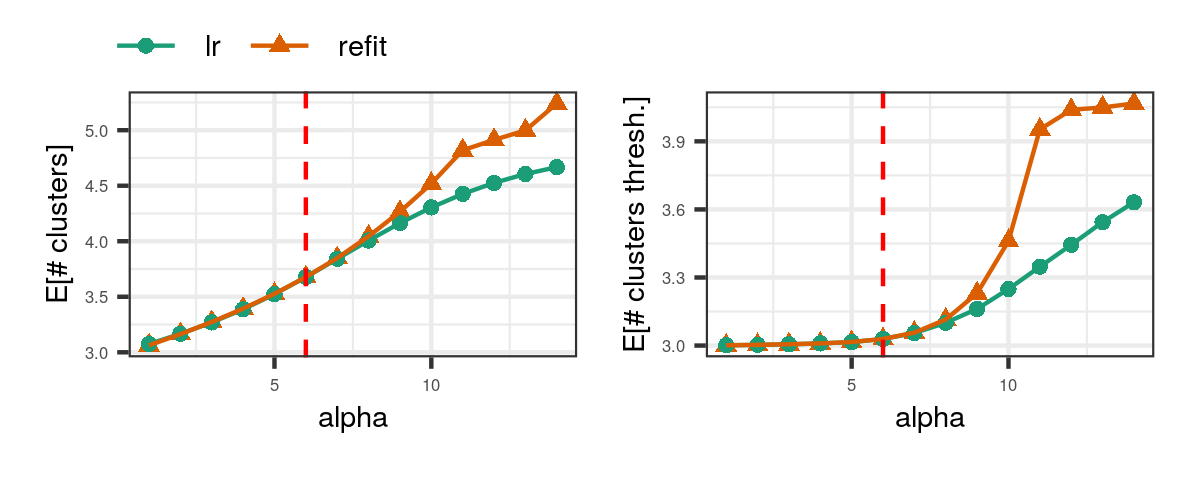
\includegraphics[width=0.980\linewidth,height=0.392\linewidth]{figure/iris_alpha_sens-1} 

}

\caption[The expected number of clusters as $\alpha$ varies in the 
the BNP-GMM fit of the iris data]{The expected number of clusters as $\alpha$ varies in the 
the BNP-GMM fit of the iris data. 
On the left is the sensitivity of the in-sample quantity.  
On the right is the the predictive quantity. 
We compute the linear approximation at $\alpha=6$ and
extrapolate the expected number of clusters using the
linear approximation (green).
We compare against the expected number of clusters obtained by refitting the model at each $\alpha$ (orange). }\label{fig:iris_alpha_sens}
\end{figure}


\end{knitrout}


% 
% - we demonstrate the utility of the influence function 
% - figure ref top three rows shows three different functional perturbations. 
% - can't really tell from densities how these will affect posterior statistic
% - but they do in fact have very different effects (in sign and size). 
% - but their effects make sense when looking at the influence function
% 
% -last row is worst-case

We next consider functional perturbations, 
and we demonstrate the ability of the influence function to 
provide guidance on the anticipated effect of perturbations 
on the posterior quantity. 
Each row of \figref{iris_fsens} explores a different 
multiplicative perturbation $\phi$ to the initial $\betadist{1, \alpha_0}$ stick distribution. 
The left column of \figref{iris_fsens} displays the perturbation $\phi$ overlayed with the prior-weighted influence function for $\gclusters$.
The perturbations are of the form 
$\log \phi(x) = e^{2(x - \mu)^2}$, with each perturbation having a 
different value of $\mu$.
Our perturbation is multiplicative in form, 
$p(\nu_k|\epsilon) = p_0(\nu_k)\phi(\nu_k)^\epsilon$.
The middle column of \figref{iris_fsens} displays the initial density,
$p_0(\nu_k) = \betadist{\nu_k\vert 1, \alpha_0}$,
along with the perturbed density,
$p(\nu_k|\epsilon = 1)$. 

Each perturbation $\phi$ produces distinct changes in the expected number of in-sample clusters $\gclusters$. 
The right column of \figref{iris_fsens} plots the differences
$\gclusters(\etaopt(\epsilon)) - \gclusters(\etaopt(0))$ 
as $\epsilon\rightarrow 1$, where $\etaopt(\epsilon)$ are variational parameters
fitted with prior stick-distribution $p(\nu_k|\epsilon)$. 
For each perturbation, the changes in are different in both sign and magnitude. 

By examining the perturbed densities $p(\nu_k|\epsilon = 1)$ alone, 
it is difficult to anticipate 
the effect of the perturbation on $\gclusters$. 
However, the sign and magnitude of the change in $\gclusters$ is well-explained by the influence function. 
When $\log\phi$ is centered at a location where the influence function is negative, the effect on $\gclusters$ is negative (top row); 
conversely, when $\log\phi$ is centered at a location where the influence function is positive, the effect on $\gclusters$ is positive (bottom row); finally, when $\log\phi$ is centered at a location where the influence is both negative and positive, the effects cancel, and the change in the posterior statistic is roughly zero (middle row). 
In each case, the linear approximation $\gclusters(\etalin(\epsilon))$
is able to capture the changes in the posterior statistic. 
In applications below, we use influence function to guide our choice of functional perturbaton and to explain why some perturbations result in greater sensitivity than others. 

Finally, we consider the 
worst-case perturbation with unit $L_\infty$ norm.
Recall that the worst-case perturbation with unit $L_\infty$ norm is a 
step-function taking on values $\pm1$ corresponding 
to the sign of the influence function (\figref{iris_worstcase} left).  
The middle column of \figref{iris_worstcase} shows the prior density perturbed by the worst-case perturbation; 
the right column shows the effect on $\gclusters$. 
We see that this worst-case perturbation has a much larger effect on
$\gclusters$ compared to the other unit $L_\infty$ norm perturbations in
\figref{iris_fsens}. 
However, even with the worst-case perturbation, 
the change in $\gclusters$ is still small;
we thus conclude that in the iris dataset $\gclusters$ appears to be a quantity insensitive to the prior. 



\begin{knitrout}
\definecolor{shadecolor}{rgb}{0.969, 0.969, 0.969}\color{fgcolor}\begin{figure}[!h]

{\centering 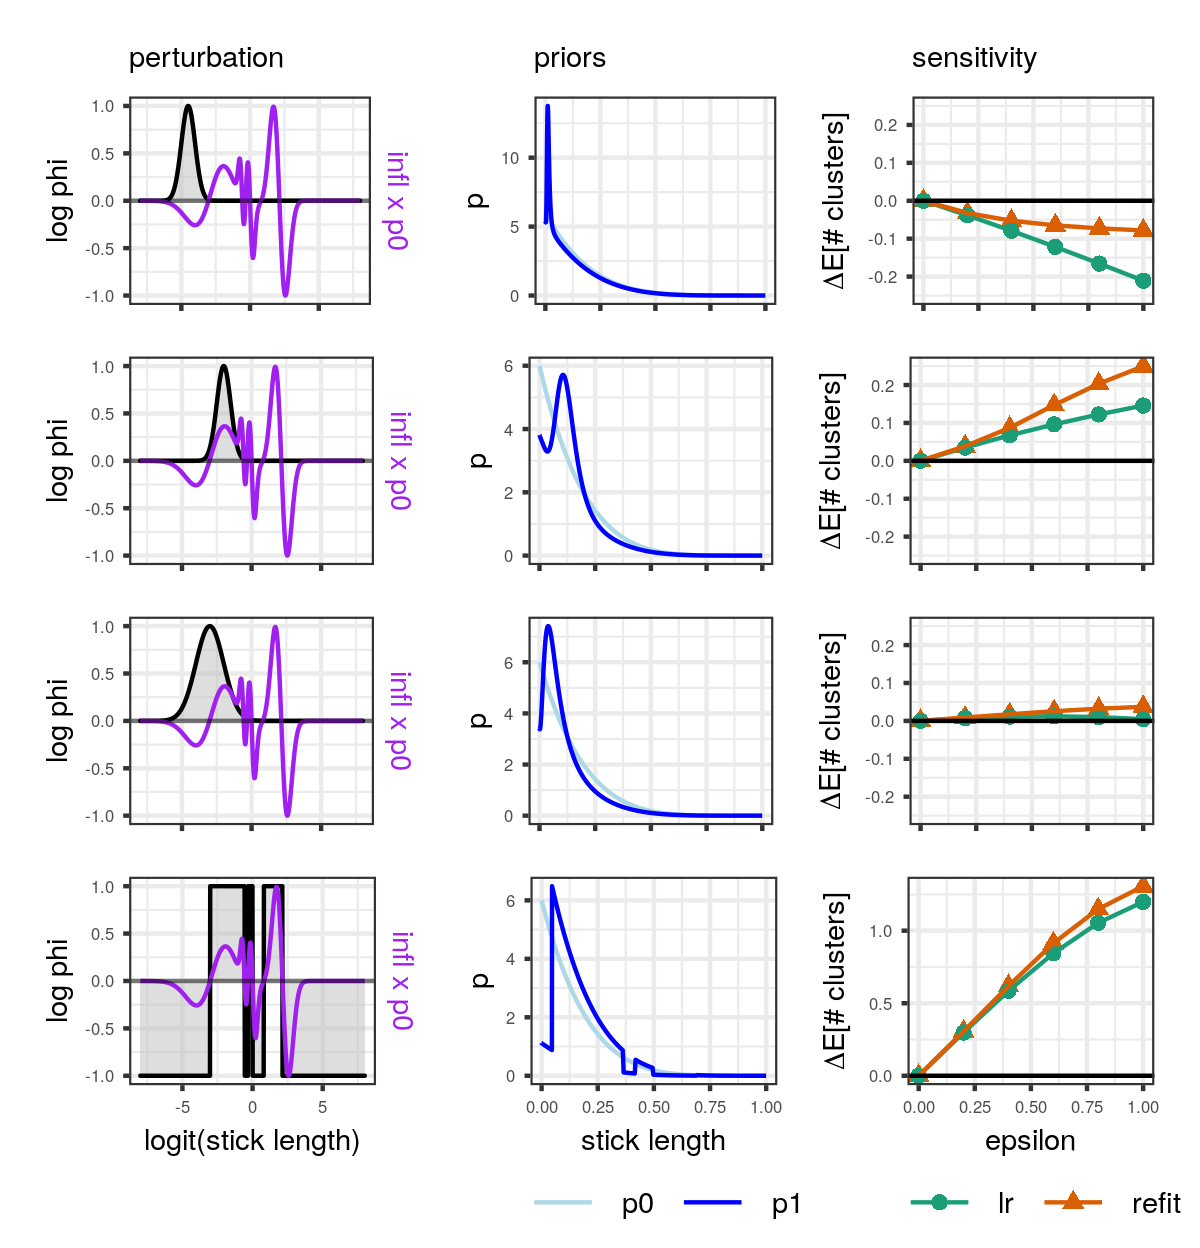
\includegraphics[width=0.980\linewidth,height=0.862\linewidth]{figure/iris_fsens-1} 

}

\caption{Sensitivity of
        the expected number of in-sample clusters in the iris dataset
        to three multiplicative perturbations with 
        unit $L_{\infty}$-norm 
        (Left) The log multiplicative perturbation $\log\phi$ in grey.        
        In purple is the prior-weighted influence function, scaled to also have 
        unit $L_{\infty}$-norm. 
        (Middle) The original prior density $p_0$ and 
        the perturbed prior density $p_1 = p_0\times \phi$. 
        (Right) The effect of the perturbation 
        on the change in expected number of clusters as a function of $\epsilon$. }\label{fig:iris_fsens}
\end{figure}


\end{knitrout}


\begin{knitrout}
\definecolor{shadecolor}{rgb}{0.969, 0.969, 0.969}\color{fgcolor}\begin{figure}[!h]

{\centering 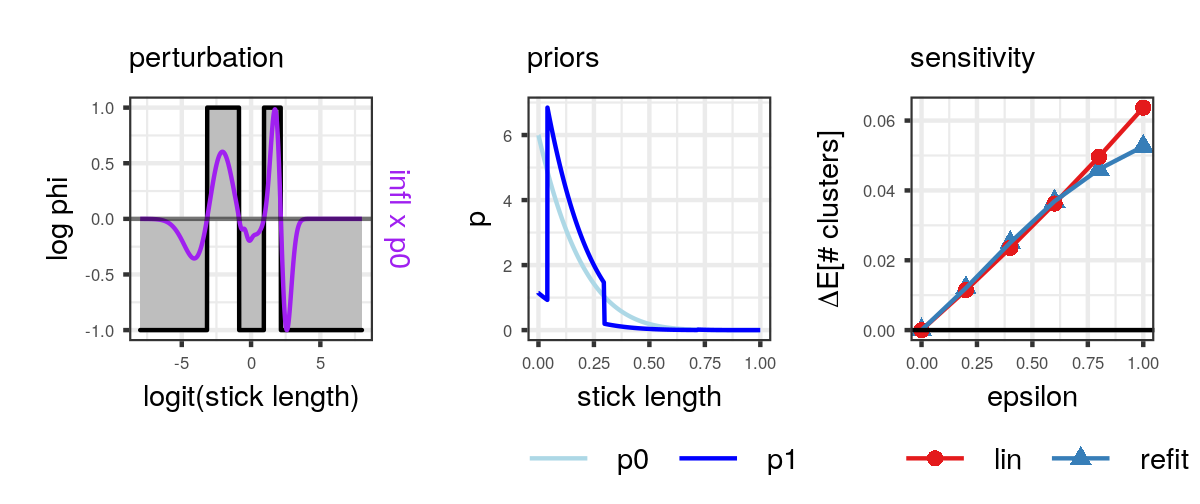
\includegraphics[width=0.980\linewidth,height=0.412\linewidth]{figure/iris_worstcase-1} 

}

\caption[Sensitivity of
        the expected number of in-sample clusters in the iris dataset
        to the worst-case multiplicative perturbations with 
        unit $L_{\infty}$-norm]{Sensitivity of
        the expected number of in-sample clusters in the iris dataset
        to the worst-case multiplicative perturbations with 
        unit $L_{\infty}$-norm.}\label{fig:iris_worstcase}
\end{figure}


\end{knitrout}

% \begin{table}[tb]
% \centering
% \caption{Compute time of results on the iris dataset. }
% \begin{tabular}{|r|r|}
%     \hline 
%     & time (seconds) \\ 
%     \hline 
%     Initial fit & sprintf('%1.2g', init_fit_time) \\
%     \hline 
%     Hessian solve for $\alpha$ sensitivity & 
%         sprintf('%1.2g', alpha_hess_time)\\
%     Linear approx. $\eta^{lin}(\alpha)$ for $\alpha = 1, ... , 16$ & 
%         sprintf('%1.2g', total_alpha_lr_time)\\
%     Refits $\eta(\alpha)$ for $\alpha = 1, ... , 16$ & 
%         sprintf('%1.2g', total_alpha_refit_time)\\
%     \hline 
%     The influence function & sprintf('%1.2g', infl_time)\\ 
%     Hessian solve for worst-case $\phi$ & 
%         sprintf('%1.2g', wc_hessian_time)\\
%     Linear approx. $\eta^{lin}(\epsilon)|_{\epsilon = 1}$
%     for worst-case $\phi$ & 
%         sprintf('%1.2g', wc_lr_time)\\
%     Refit $\eta(\epsilon)|_{\epsilon = 1}$ for worst-case $\phi$ & 
%         sprintf('%1.2g', wc_refit_time)\\ 
%     \hline 
% \end{tabular}
% \end{table}

